\section{Retained v3 Evaluation: Historical Evidence}\label{app:v3evidence}
All results in this appendix were recorded in v3. ``Fresh below distinguishes its actual checker executions from its v2 replay, not new v4 runs. No outcomes in this appendix are pooled with the v4 transport or v5 layout studies.
\subsection{Questions, frozen protocols, and provenance}
The evaluation asks four questions: Does learned display order recover savings lost to arbitrary registries? Can online selection pay for its own migrations under drift? Do results survive actual source checking? What overhead remains when the verifier is called by a real agent harness?

The v3 experimental contract fixes four synthetic families, seeds 0--19, training/validation/evaluation sizes, packet widths, catalogue policies, and online parameters before their runs. Ordering uses $n=64$, 256 training, 128 validation, and 512 evaluation episodes per seed. Online evaluation uses 2,048 events per stream and $\eta=.5,\alpha=.01$. We retain these parameters after observing unfavorable results. All synthetic random seeds and realized waves are stored. Error bars are percentile bootstrap intervals over 20 paired \emph{seed-level} measurements, not over thousands of correlated inner events; 10,000 bootstrap resamples use seed 94001. These are descriptive 95\% intervals, not simultaneous guarantees over every comparison.

The source-study lineage is explicit. The artifact retains v2's 121 source interventions: 45 training, 43 development, and 33 later confirmation cases. One development execution timed out and remains unknown. This revision reuses those outcome records for training, validation, and \emph{retrospective replay}; it does not relabel the 33 published cases as new unseen v3 data. It then runs 24 fresh paired candidate checks on 12 selected archived interventions, plus trusted baselines and restored-source checks. Finally it adds nine actual runtime episodes on a new non-arithmetic I/O fixture. Repetition, provenance, and scope are different across these studies and are not pooled into a single success-rate statistic.

\subsection{RQ1: Ordering robustness and negative controls}
Shuffled-cluster workloads generate eight-check groups in a randomly permuted semantic registry, with a 12\% probability of one additional check. Independent workloads activate each check with probability $8/n$. Singleton workloads use a Zipf-like exponent 1.2; global workloads activate all checks. Every reported ordering cost includes a fresh full-tree construction. The baseline ``original DP'' uses the same exact compiler and full-wave observations but preserves registry order; ``fixed8'' is the compact bottom-up eight-child tree. Selection uses only the separate validation cohort.

\begin{table}[t]\centering\small
\caption{Archived v3. Mean paired byte reduction in percent; positive is better. Brackets are seed-bootstrap 95\% intervals. Each row uses 20 seeds and 512 held-out episodes per seed. Initialization is included.}\label{tab:ordering}
\begin{tabular}{@{}lrr@{}}\toprule
Workload & Versus original-order DP & Versus fixed8\\\midrule
\csname @@input\endcsname generated/ordering_rows.tex 
\bottomrule\end{tabular}
\end{table}

On shuffled clusters, the selected learned order reduces cost by 26.38\% relative to original-order DP and 28.46\% relative to fixed8. The independent control has a small negative point estimate whose interval crosses zero. Under singleton updates, the original-order compiler already captures the relevant per-check skew, and the selected proposals tie it. Global refreshes also tie. Thus the result is not ``reordering always helps''; it is recovery of avoidable serialization cost when the registry is misaligned with correlated completion groups.

\begin{figure}[t]\centering
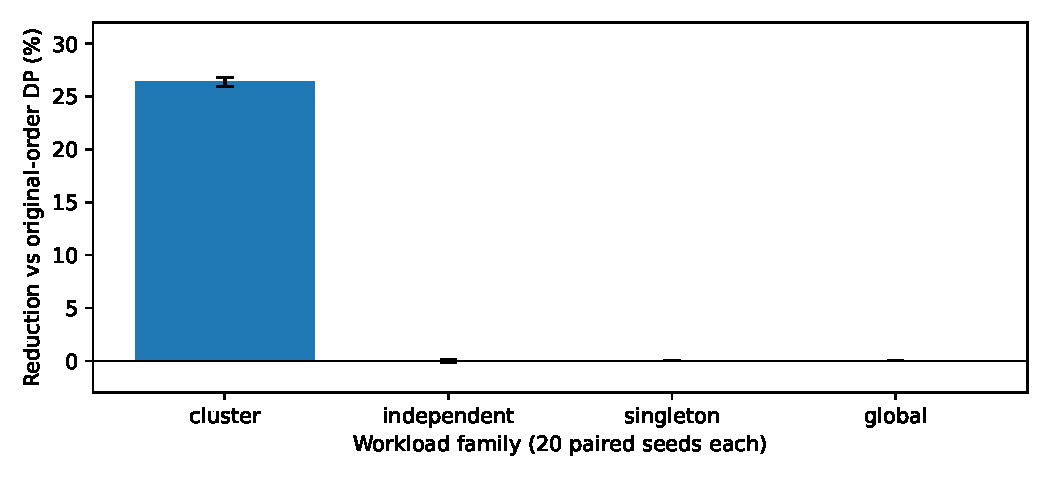
\includegraphics[width=.88\linewidth]{figures/ordering.pdf}
\caption{Archived v3. Ordering improves the structured shuffled case, not every workload. The zero line is the unchanged original-order compiler. The figure shows the same data as Table~\ref{tab:ordering}.}
\end{figure}

\paragraph{Construction cost and scale.}
With single-threaded BLAS, fitting all three proposals on 128 calibration episodes took 0.075, 0.356, 1.449, 3.637, and 18.435 seconds at $n=32,64,128,256,512$, respectively. These are single construction measurements, not averaged throughput estimates. All produced packet maxima were 3,072 bytes. The cubic compiler should be run at controlled decision points, not after every small edit. The experiment establishes bounded packet size up to 512 \emph{checks}, not 512 simultaneous LLM workers or constant total computation.

\subsection{RQ2: Drift, switching costs, and competing policies}
Four calibration regimes are fixed before evaluation: original clusters, permuted clusters, independent activity, and global activity. Their compiled layouts form a small frozen catalogue, deduplicated by manifest hash. The ``frozen'' comparator is chosen using original-cluster calibration. Long shift consists of four 512-event phases: original clusters, permuted clusters, independent activity, and global activity. Rapid shift alternates original/permuted clusters every eight events. Stationary and global streams are controls.

These are persistent refresh traces: per-tick costs do not include a new candidate's unconditional full construction. Every actual topology change does include canonical manifest serialization plus a full cold reconstruction. The event's wave is observed only after choosing the current layout. No future phase boundary is supplied to the selector. All catalogue losses are recomputed from that same wave; the measured scoring and controller CPU time are stored separately.

We compare coupled fixed-share with independent sampling of the same weights, zero-share coupling, a deterministic 64-event priced-window heuristic, and a last-event greedy rule that ignores switching price when deciding but is still charged its realized migrations. A clairvoyant switching-cost dynamic program is labeled an offline comparator, not a deployable policy.

\begin{table}[t]\centering\small
\caption{Archived v3. Mean seed-level total charged cost divided by frozen-layout cost; lower is better. All migration bytes are included. CS: coupled share; IS: independent share; C0: zero-share coupling; PW: priced window; GU: unpriced greedy; oracle: clairvoyant switching comparator.}\label{tab:online}
\begin{tabular}{@{}lrrrrrr@{}}\toprule
Stream & CS & IS & C0 & PW & GU & Oracle\\\midrule
\csname @@input\endcsname generated/online_rows.tex 
\bottomrule\end{tabular}
\end{table}

Coupled share achieves a long-shift ratio of 0.845, with 95\% interval [0.834, 0.856], equivalent to a mean 15.52\% reduction. Independent sampling loses enough migration bytes to exceed the frozen comparator, despite using the same evolving marginal weights. This validates the importance of temporal coupling, not a claim of a new weighted-majority method.

The negative results are consequential. Coupled share regresses by 7.88\% on stationary streams and 16.45\% on rapidly alternating streams; its mean switch counts are 4.55 and 111.65, respectively. The simple priced-window rule is cheaper in both these settings and in long shift. The theorem-backed policy is therefore not the empirical winner. Its value is an explicit, auditable service/migration accounting and a guarantee under stated assumptions, not universal dominance. The global control exhibits no cost differences among layouts, so maximal coupling makes zero switches, whereas independent draws incur avoidable installation cost.

\begin{figure}[t]\centering
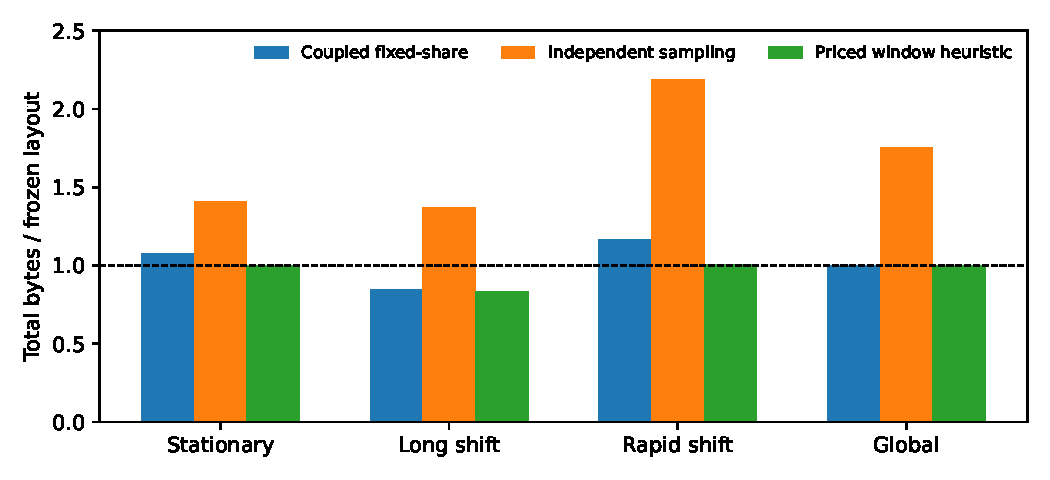
\includegraphics[width=.92\linewidth]{figures/online.pdf}
\caption{Archived v3. Total service plus migration cost. The dashed line is frozen-layout cost. Reduced switching matters, but the coupled policy still loses under stationary and rapid-shift conditions.}
\end{figure}

\subsection{RQ3: Existing source projects and fresh executions}
The retained projects are NetworkX, Toolz, and the Future Code runtime, with scoped registries of 170, 148, and 138 checks. The same v2 intervention-conditioned execution ranker is used for every layout; only certificate display order changes. Training uses complete recorded mutation outcomes. A separate development cohort selects among original, spectral, and cluster layouts; clustering is selected for all three projects. A deterministically shuffled-registry DP exposes sensitivity to an arbitrary order.

\begin{table}[t]\centering\small
\caption{Archived v3. Retrospective replay on v2's 33 published confirmation cases. Values are aggregate byte reductions in percent, including per-candidate initialization. This is not newly executed or untouched v3 generalization evidence.}\label{tab:replay}
\begin{tabular}{@{}lrrrrr@{}}\toprule
Project & Checks & Cases & vs original DP & vs fixed8 & vs shuffled DP\\\midrule
\csname @@input\endcsname generated/replay_rows.tex 
\bottomrule\end{tabular}
\end{table}

To check replay mechanics against actual execution, we freeze the first four lexicographically ordered confirmation IDs per project, independently of the new savings, then execute each candidate with fixed8 and the validation-selected layout. Mode order alternates by case. The exact original source hashes, mutation spans, replacement text, resulting hashes, orders, reports, and packet streams are retained. This deterministic small cohort is not a representative sample of all defects; some cases share source locations or produce unchanged test outcomes.

\begin{table}[t]\centering\small
\caption{Archived v3. Fresh paired executions, four candidates per project and mode. Bytes are actual emitted streams; seconds are summed outer-wrapper durations, including snapshotting and report writing. Check execution order is identical within each pair.}\label{tab:fresh}
\begin{tabular}{@{}lrrrrr@{}}\toprule
 & \multicolumn{2}{c}{Certificate KiB} & Reduction & \multicolumn{2}{c}{Outer duration (s)}\\
Project & fixed8 & learned & (\%) & fixed8 & learned\\\midrule
\csname @@input\endcsname generated/fresh_rows.tex 
\bottomrule\end{tabular}
\end{table}

All 24 fresh candidate decisions match their recorded full-suite oracle verdicts. The three trusted baselines and three scripted restorations pass. The two layouts execute the same number of checks in each pair, and the independent auditor reproduces the measured packet bytes from the actual completion sequence. Across the 12 pairs, aggregate wrapper time is 39.69 seconds for fixed8 and 39.77 seconds for learned layouts. This is essentially unchanged, not a wall-clock improvement corresponding to the byte reductions. Subprocess startup, imports, snapshot acquisition, and tests dominate this small execution setting.

\subsection{RQ4: Actual harness integration and I/O behavior}
The new fixture contains an idempotent SQLite ledger, bounded HTTP JSON transport, and an integration service. Its 40 checks exercise disk-backed transactions, duplicate event handling, conflicting idempotency keys, rejected writes, actual loopback HTTP requests, malformed and oversized responses, HTTP errors, and end-to-end ingestion. The tests use real SQLite and socket I/O; the failures and repaired source content are scripted. Network delays, remote services, and nondeterministic production systems are not represented.

A real Future Code supervisor receives a root coordinator task that delegates to two children with disjoint write scopes. Each child reads its module, submits an incorrect implementation, receives an executable rejection, then submits the known correct implementation. The parent verifies integration. A local HTTP server supplies the scripted model actions and injects one HTTP 503 before a successful retry. The model-response script is identical across gate modes. Provider usage is absent and recorded as unknown.

Three repetitions rotate mode order among direct pytest, strict fixed8, and strict learned-layout gates. The strict variants use trusted baseline contracts outside candidate scopes and the actual bridge subprocess. Their layout calibration is an explicit predeployment completion-wave fixture, not training on evaluated episode outcomes. Setup/contract fitting is recorded separately from active episode time. The small fixture is intentionally capable of showing no layout benefit.

\begin{table}[t]\centering\small
\caption{Archived v3. Nine actual harness episodes, three per mode. Duration runs from supervisor startup through completion and shutdown. Prompt bytes include retries and all worker calls, not hosted tokens. Certificate bytes are not applicable for direct pytest.}\label{tab:harness}
\begin{tabular}{@{}lrrrrr@{}}\toprule
Mode & Runs & Median s & Range s & Mean cert. KiB & Mean prompt KiB\\\midrule
\csname @@input\endcsname generated/harness_rows.tex 
\bottomrule\end{tabular}
\end{table}

All nine episodes complete the three-task graph with an observed peak of two active workers, reject at least the two intentionally incorrect candidates, and recover from the injected outage. All final source modules equal the scripted correct inputs. Strict modes produce 97,920 certificate bytes per episode and tie each other. Their median active time is about 18.1 seconds versus 13.0 seconds for direct gates. This roughly five-second premium buys the additional source/contract checks and evidence materialization; it is not an optimization speedup.

The maximum observed aggregate message-content size per HTTP request is 6,902 UTF-8 bytes, below the runtime's 16,384-byte input cap. Mean total context-construction time is 6.3--7.2 milliseconds per episode; total prompts are about 70--71 KiB. These measurements do not imply a statistically established prompt reduction, billing reduction, or improvement in model cognition. Only two simultaneous workers are measured here.

\subsection{Software verification and independent audit}
The full prototype suite passes 187 tests, including 43 new v3 tests beyond v2's 144. Separately, the vendored Future Code runtime passes all 263 of its own tests. New cases cover invalid and duplicate permutations, disconnected affinity graphs, degenerate spectral choices, exhaustive small-order comparisons, pairwise information loss, coupled marginal distributions, checkpoint continuation, choice-before-observation enforcement, priced migration, canonical-ID remapping, stale tickets, delayed evidence, contradictory records, bridge subprocesses, and independent-auditor tamper rejection.

The audit imports neither the compiler nor producer cost helpers. It reconstructs all 80 ordering workloads, all 80 online streams (163,840 events), the 33 archived replay cases, 24 fresh paired runs, and nine harness episode records. It also checks 63 actual binary packet streams containing 2,305 packets and independently recomputes 32 reported bootstrap comparisons. A label mismatch that initially left an empty cohort in the draft summary was detected and corrected; summaries now reject missing cohorts instead of treating absence as zero cost. No erroneous draft statistic is included in the paper. These checks are independent implementation paths, not an external replication or security certification.
